%--------------------------------------
%CANEVAS
%--------------------------------------

%--------------------------------------
%appel de la classe de document et de ses options
%--------------------------------------
\PassOptionsToPackage{french}{translator}

\documentclass[10pt]{beamer}

\usepackage{AOCDTF_diaporama}

%--------------------------------------
%données du document
%--------------------------------------

\title{La matière} %inscrire le nom de la matière ici

\subtitle{Le cours} %inscrire le nom du cours ici

\date{
\begin{minipage}{0.49\textwidth}
\footnotesize{Édition \the\year.\the\month}
\end{minipage}
\hfill
\begin{minipage}{0.49\textwidth}
\raggedleft{\footnotesize{Prénom \textsc{Nom}}} %inscrire le nom de l'auteur ici
\end{minipage}}

\institute{
\begin{center}
\begin{large}
\textsc{La formation} %inscrire le nom de la formation ici
\end{large}
\end{center}
\vspace{0.7cm}
\begin{minipage}{0.65\textwidth}
Association Ouvrière des Compagnons du Devoir et du tour de France
\end{minipage}
\hfill
\begin{minipage}{0.3\textwidth}
	\begin{flushright}

\includegraphics[height=0.7cm]{logo_compagnons}
\end{flushright}
\end{minipage}

\vspace{0.7cm}

\begin{minipage}{0.3\textwidth}
	\begin{flushleft}

\includegraphics[height=0.7cm]{blason_MTA}
\end{flushleft}
\end{minipage}
\hfill
\begin{minipage}{0.65\textwidth}
\begin{flushright}
Le corps de métier %inscrire le corps de métier ici
\end{flushright}
\end{minipage}}

%--------------------------------------
%corps du document
%--------------------------------------

\begin{document}

\maketitle

\begin{frame}{Table des matières}
  \setbeamertemplate{section in toc}[sections numbered]
  \tableofcontents[hideallsubsections]
\end{frame}

\section{Une première section}

\begin{frame}[fragile]{Titre de la diapositive 1}
    \metroset{block=fill} %bloc rempli
    \begin{block}{Titre du bloc}
        Contenu du bloc
    \end{block}
    \begin{itemize}[<+(1)- | alert@+(1)>] %liste avec une slide qui met en évidence chaque terme de la liste (apparait à la deuxième slide)
		\item Un premier truc \alert<5>{\only<5>{ (truc en évidence à la cinquième slide)}}  
		\item Un deuxième truc
		\item Un troisième truc
    \end{itemize}
\onslide+<5->{ %partie qui apparait à la cinquième slide sans effacer ce qui apparait sur les slides précédentes         
    \metroset{block=fill}
    \begin{block}{Titre du bloc}
Contenu du bloc
     \end{block}}  
\end{frame}

\begin{frame}[fragile]{Titre de la diapositive 2}
    \metroset{block=fill} %bloc rempli
    \begin{block}{Titre du bloc}
    \begin{itemize}[<+(1)- | alert@+(1)>] %liste avec une slide qui met en évidence chaque terme de la liste (apparait à la deuxième slide)
      	\item Un premier truc
		\item Un deuxième truc
		\item Un troisième truc
    \end{itemize}
    \end{block}
\onslide+<5->
    \metroset{block=fill}
    \begin{block}{Titre du bloc}
    \begin{itemize}[<+(2)- | alert@+(2)>] %liste avec une slide qui met en évidence chaque terme de la liste (apparait à la sixième slide)
      	\item Un premier truc
		\item Un deuxième truc
    \end{itemize}
    \end{block}
\end{frame}

\begin{frame}[fragile]{Titre de la diapositive 3} %grosse prise de tête pour inclure du code dans une diapositive
Texte en haut de la diapositive 3
\begin{verbnobox}[\tiny]
\begin{frame}[fragile]{Titre de la diapositive 3}
Texte en haut de la diapositive 3
\begin{Verbnobox}[\tiny]
\begin{frame}[fragile]{Titre de la diapositive 3}
Texte en haut de la diapositive 3
\end{frame}\end{Verbnobox}
\end{frame}\end{verbnobox}
\end{frame}


\begin{frame}[fragile]{Titre de la diapositive 4}
\begin{center}
\copyrightbox[b]{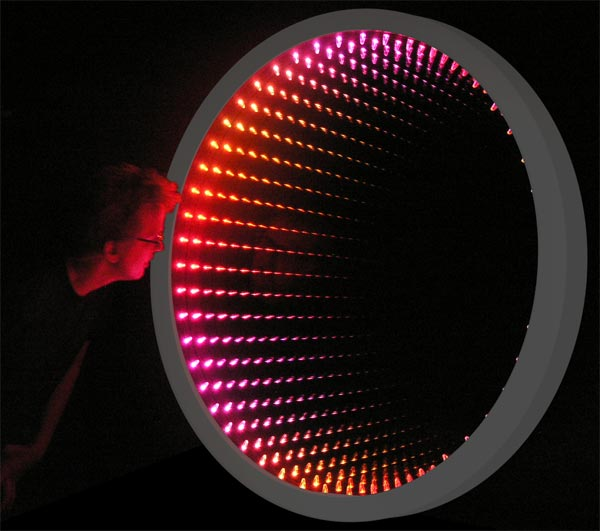
\includegraphics[scale=0.3]{infinite_mirror.jpg}}{\scriptsize{http://lightenergystudio.com/RGBinfinitymirror.html}} %une image avec son copyright
\end{center}
\end{frame}


\begin{frame}[fragile]{Titre de la diapositive 5} %diapositive avec GANTT
\onslide+<1->
\setcounter{myWeekNum}{40}
\ganttset{calendar week text={\myWeek{}}}	
\begin{ganttchart}[
	expand chart=\textwidth,
	vgrid={*{6}{draw=none}, dotted},
	y unit chart=0.7cm,
 	title/.append style={fill=black!10},
	bar height=.2,
	title label font=\tiny,
	group label font=\bfseries\tiny,
	bar label font=\tiny,
	time slot format=isodate,
	]{2020-10-01}{2021-03-31}

\ganttset{calendar week text={\myWeek{}}}	
\gantttitlecalendar{month=name, week=41 day} \\

\onslide+<2->

\ganttgroup{Un premier groupe de tâches}{2020-10-01}{2021-02-17} \\

\ganttbar{tâche 1}{2020-10-01}{2020-12-12} \\

\ganttbar{tâche 2}{2020-12-12}{2021-02-17} \\

\onslide+<3->
\ganttgroup{Un deuxième groupe de tâches}{2021-02-18}{2021-03-14} \\

\ganttbar{tâche 1}{2021-02-18}{2021-03-03} \\

\ganttbar{tâche 2}{2021-03-03}{2021-03-14} \\

\onslide+<4>
\ganttgroup{Un troisième groupe de tâches}{2021-03-15}{2021-03-31} \\

\end{ganttchart}

\end{frame}

\section{Une deuxième section}

\begin{frame}{Titre de la diapositive 6}
\onslide+<1->

 \metroset{block=fill} %bloc rempli
    \begin{block}{Titre du bloc}
        Contenu du bloc
    \end{block}

\onslide+<2->

 \metroset{block=fill} %bloc rempli
    \begin{block}{Titre du bloc}
        Contenu du bloc
    \end{block}
\onslide+<3->

 \metroset{block=fill} %bloc rempli
    \begin{block}{Titre du bloc}
        Contenu du bloc
    \end{block}

\onslide+<4->

 \metroset{block=fill} %bloc rempli
    \begin{block}{Titre du bloc}
        Contenu du bloc
    \end{block}

\end{frame}

\begin{frame}{Titre de la diapositive 7}
    
\onslide+<1->

\metroset{block=fill}
    \begin{block}{Titre du bloc}
\begin{itemize}[<+- | alert@+>]
      	\item Un premier truc
		\item Un deuxième truc
		\item Un troisième truc
\end{itemize}
    \end{block}
    
\onslide+<4->

 \metroset{block=fill} %bloc rempli
    \begin{block}{Titre du bloc}
        Contenu du bloc
    \end{block}
    
    \onslide+<5->

\metroset{block=fill}
    \begin{block}{Titre du bloc}
\begin{itemize}[<+(1)- | alert@+(1)>]
      	\item Un premier truc
		\item Un deuxième truc
		\item Un troisième truc
\end{itemize}
    \end{block}

\end{frame}

\begin{frame}[fragile]{Titre de la diapositive 8}
    \begin{itemize}[<+- | alert@+>]
      	\item Un premier truc
		\item Un deuxième truc
    \end{itemize}
\end{frame}

\section{Une troisième section}

\begin{frame}{Titre de la diapositive 9}
\onslide+<1->

 \metroset{block=fill} %bloc rempli
    \begin{block}{Titre du bloc}
        Contenu du bloc
    \end{block}

\onslide+<3->

 \metroset{block=fill} %bloc rempli
    \begin{block}{Titre du bloc}
        Contenu du bloc
    \end{block}
\onslide+<4->

 \metroset{block=fill} %bloc rempli
    \begin{block}{Titre du bloc}
        Contenu du bloc
    \end{block}

\onslide+<5->

 \metroset{block=fill} %bloc rempli
    \begin{block}{Titre du bloc}
        Contenu du bloc
    \end{block}

\end{frame}

\begin{frame}{Titre de la diapositive 10}
    
\onslide+<1->

\metroset{block=fill}
    \begin{block}{Titre du bloc}
\begin{itemize}[<+- | alert@+>]
      	\item Un premier truc
		\item Un deuxième truc
		\item Un troisième truc
\end{itemize}
    \end{block}
    
\onslide+<4->

 \metroset{block=fill} %bloc rempli
    \begin{block}{Titre du bloc}
        Contenu du bloc
    \end{block}
    \onslide+<5->

\metroset{block=fill}
    \begin{block}{Titre du bloc}
\begin{itemize}[<+(1)- | alert@+(1)>]
      	\item Un premier truc
		\item Un deuxième truc
		\item Un troisième truc
\end{itemize}
    \end{block}

\end{frame}

\begin{frame}[fragile]{Titre de la diapositive 11}
\begin{itemize}[<+- | alert@+>]
      	\item Un premier truc
		\item Un deuxième truc
		\item Un troisième truc
\end{itemize}
    	\onslide+<3->
    \begin{center}
            \copyrightbox[b]{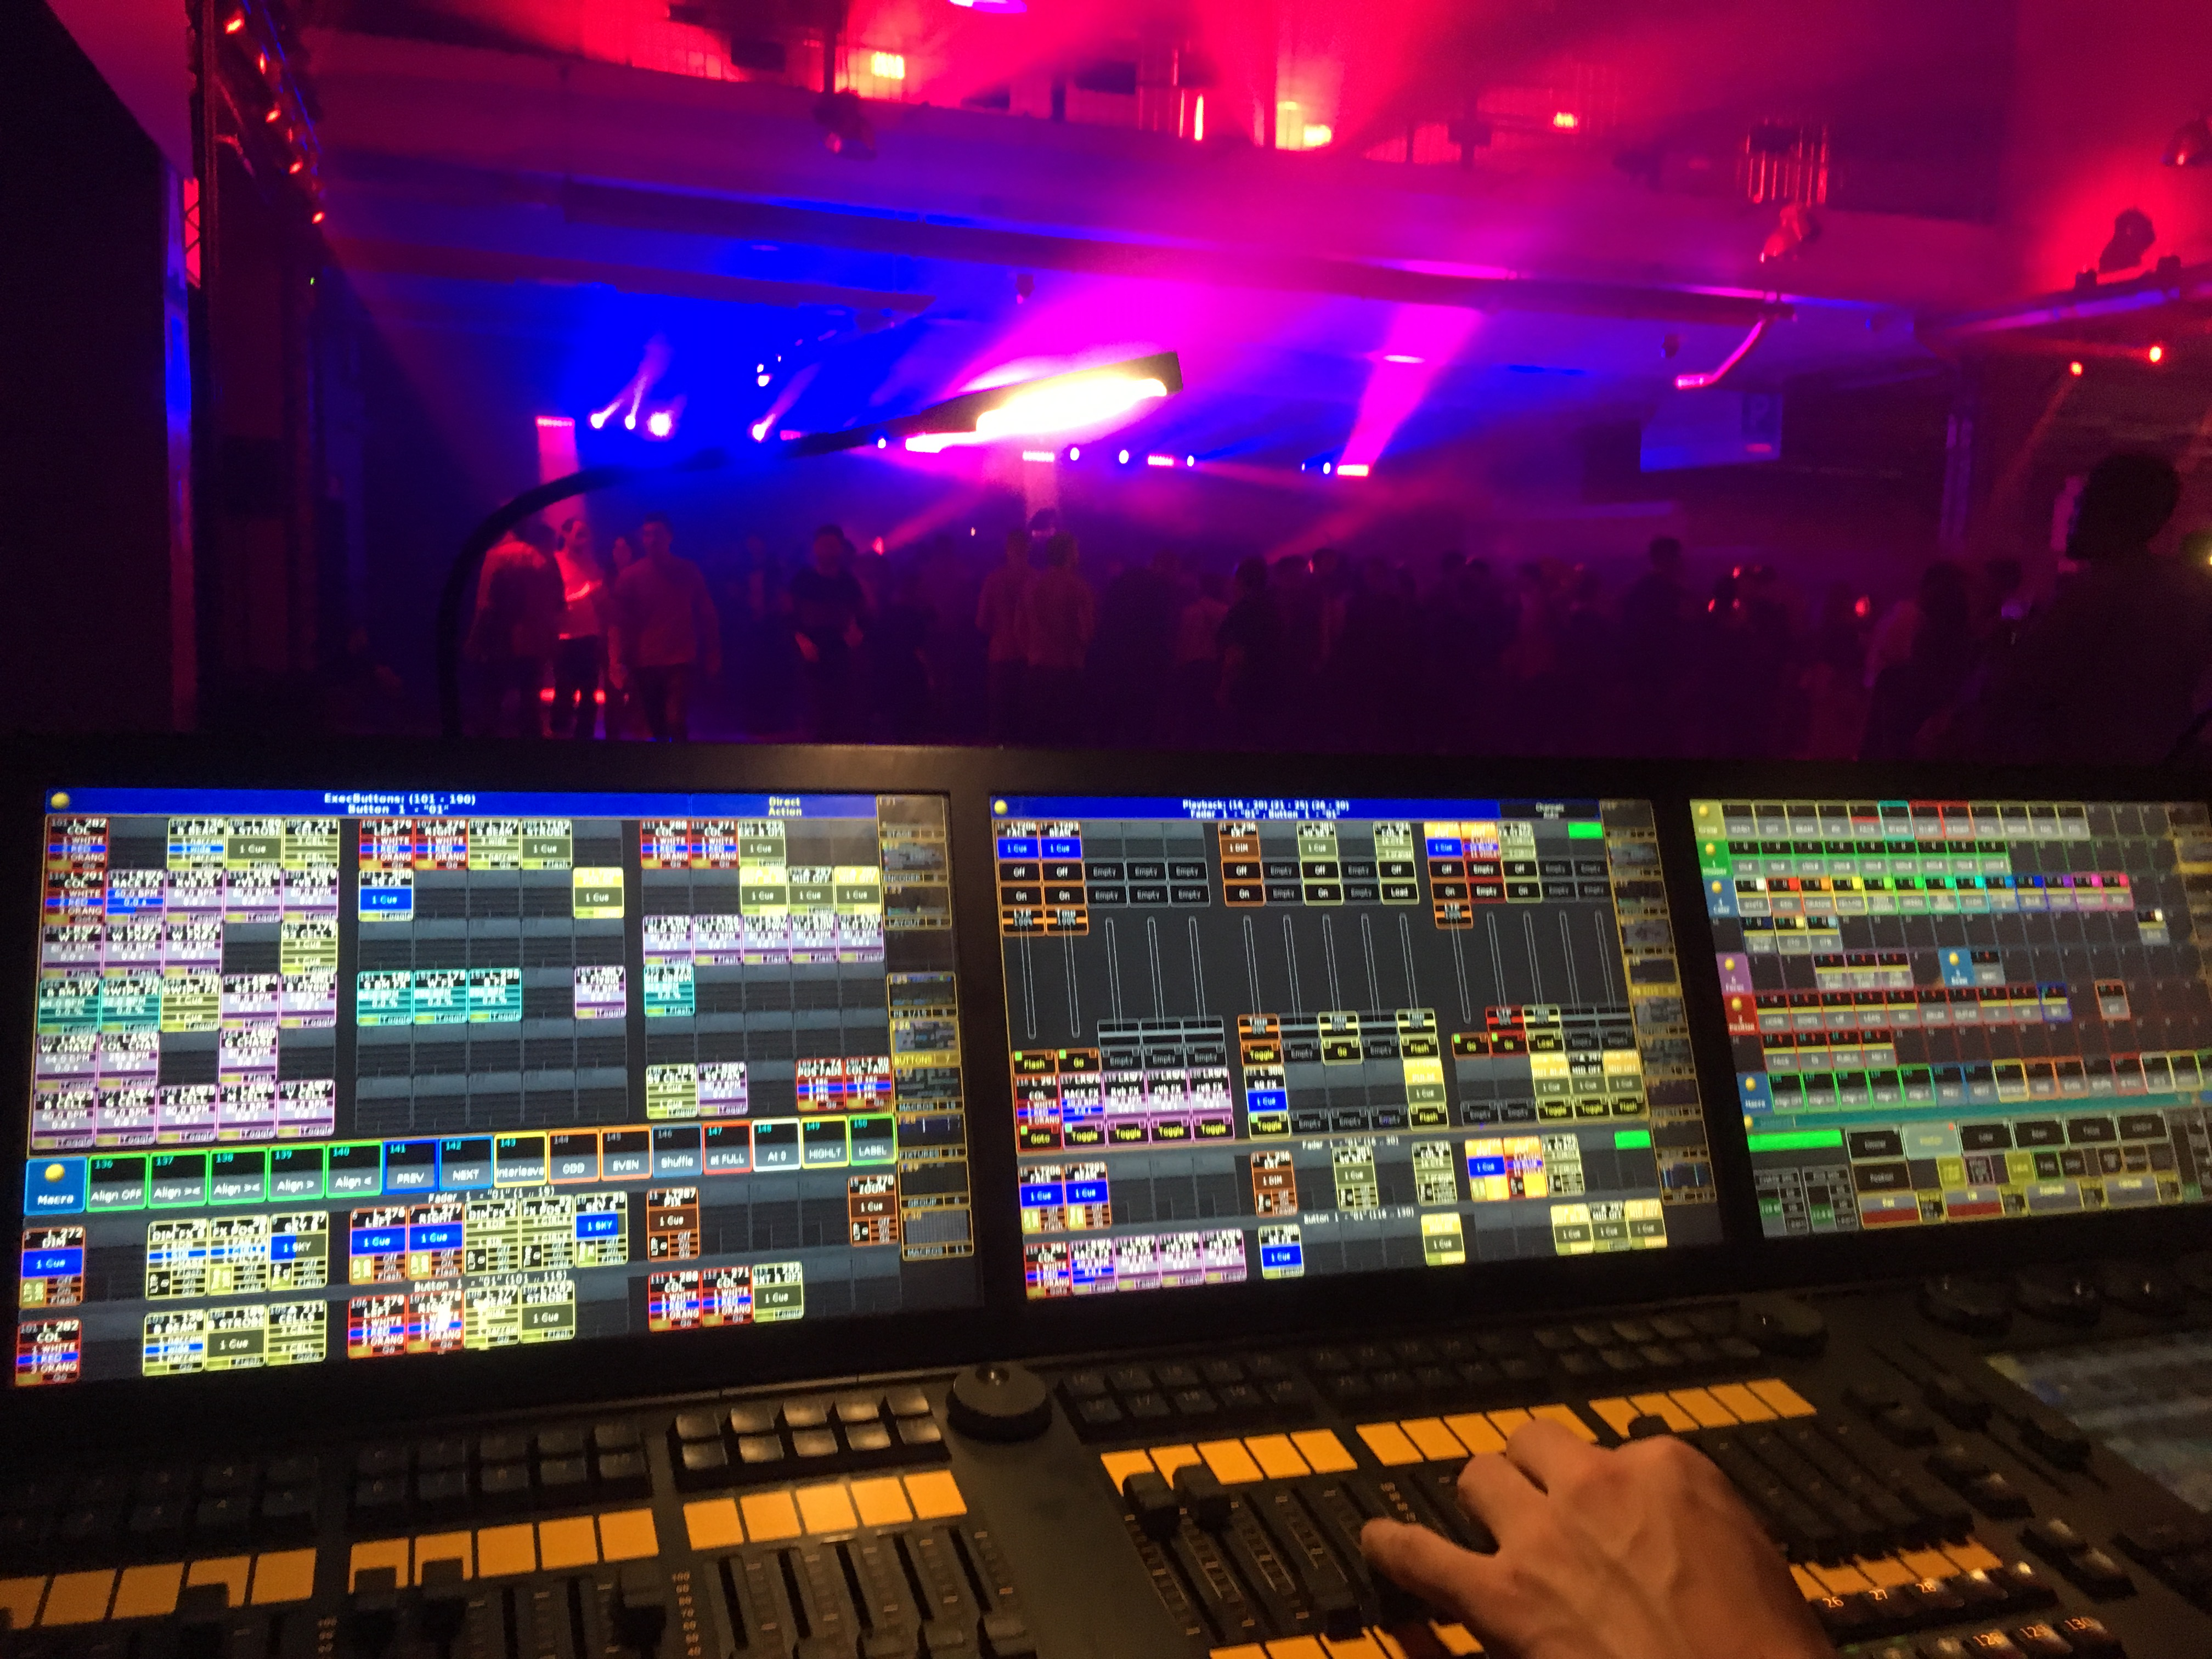
\includegraphics[scale=0.05]{platine_lumiere.jpeg}}{Image détenue par l'auteur}
	\end{center}
\end{frame}

\begin{frame}[fragile]{Titre de la diapositive 13}
Texte haut de diapositive
\begin{itemize}
	\onslide+<2->{\item un premier truc} %sur la slide deux
	\onslide+<3->{\item un deuxième truc} %sur la slide trois
\end{itemize}
	\vspace{0.5cm}
	\onslide+<2->{\copyrightbox[b]{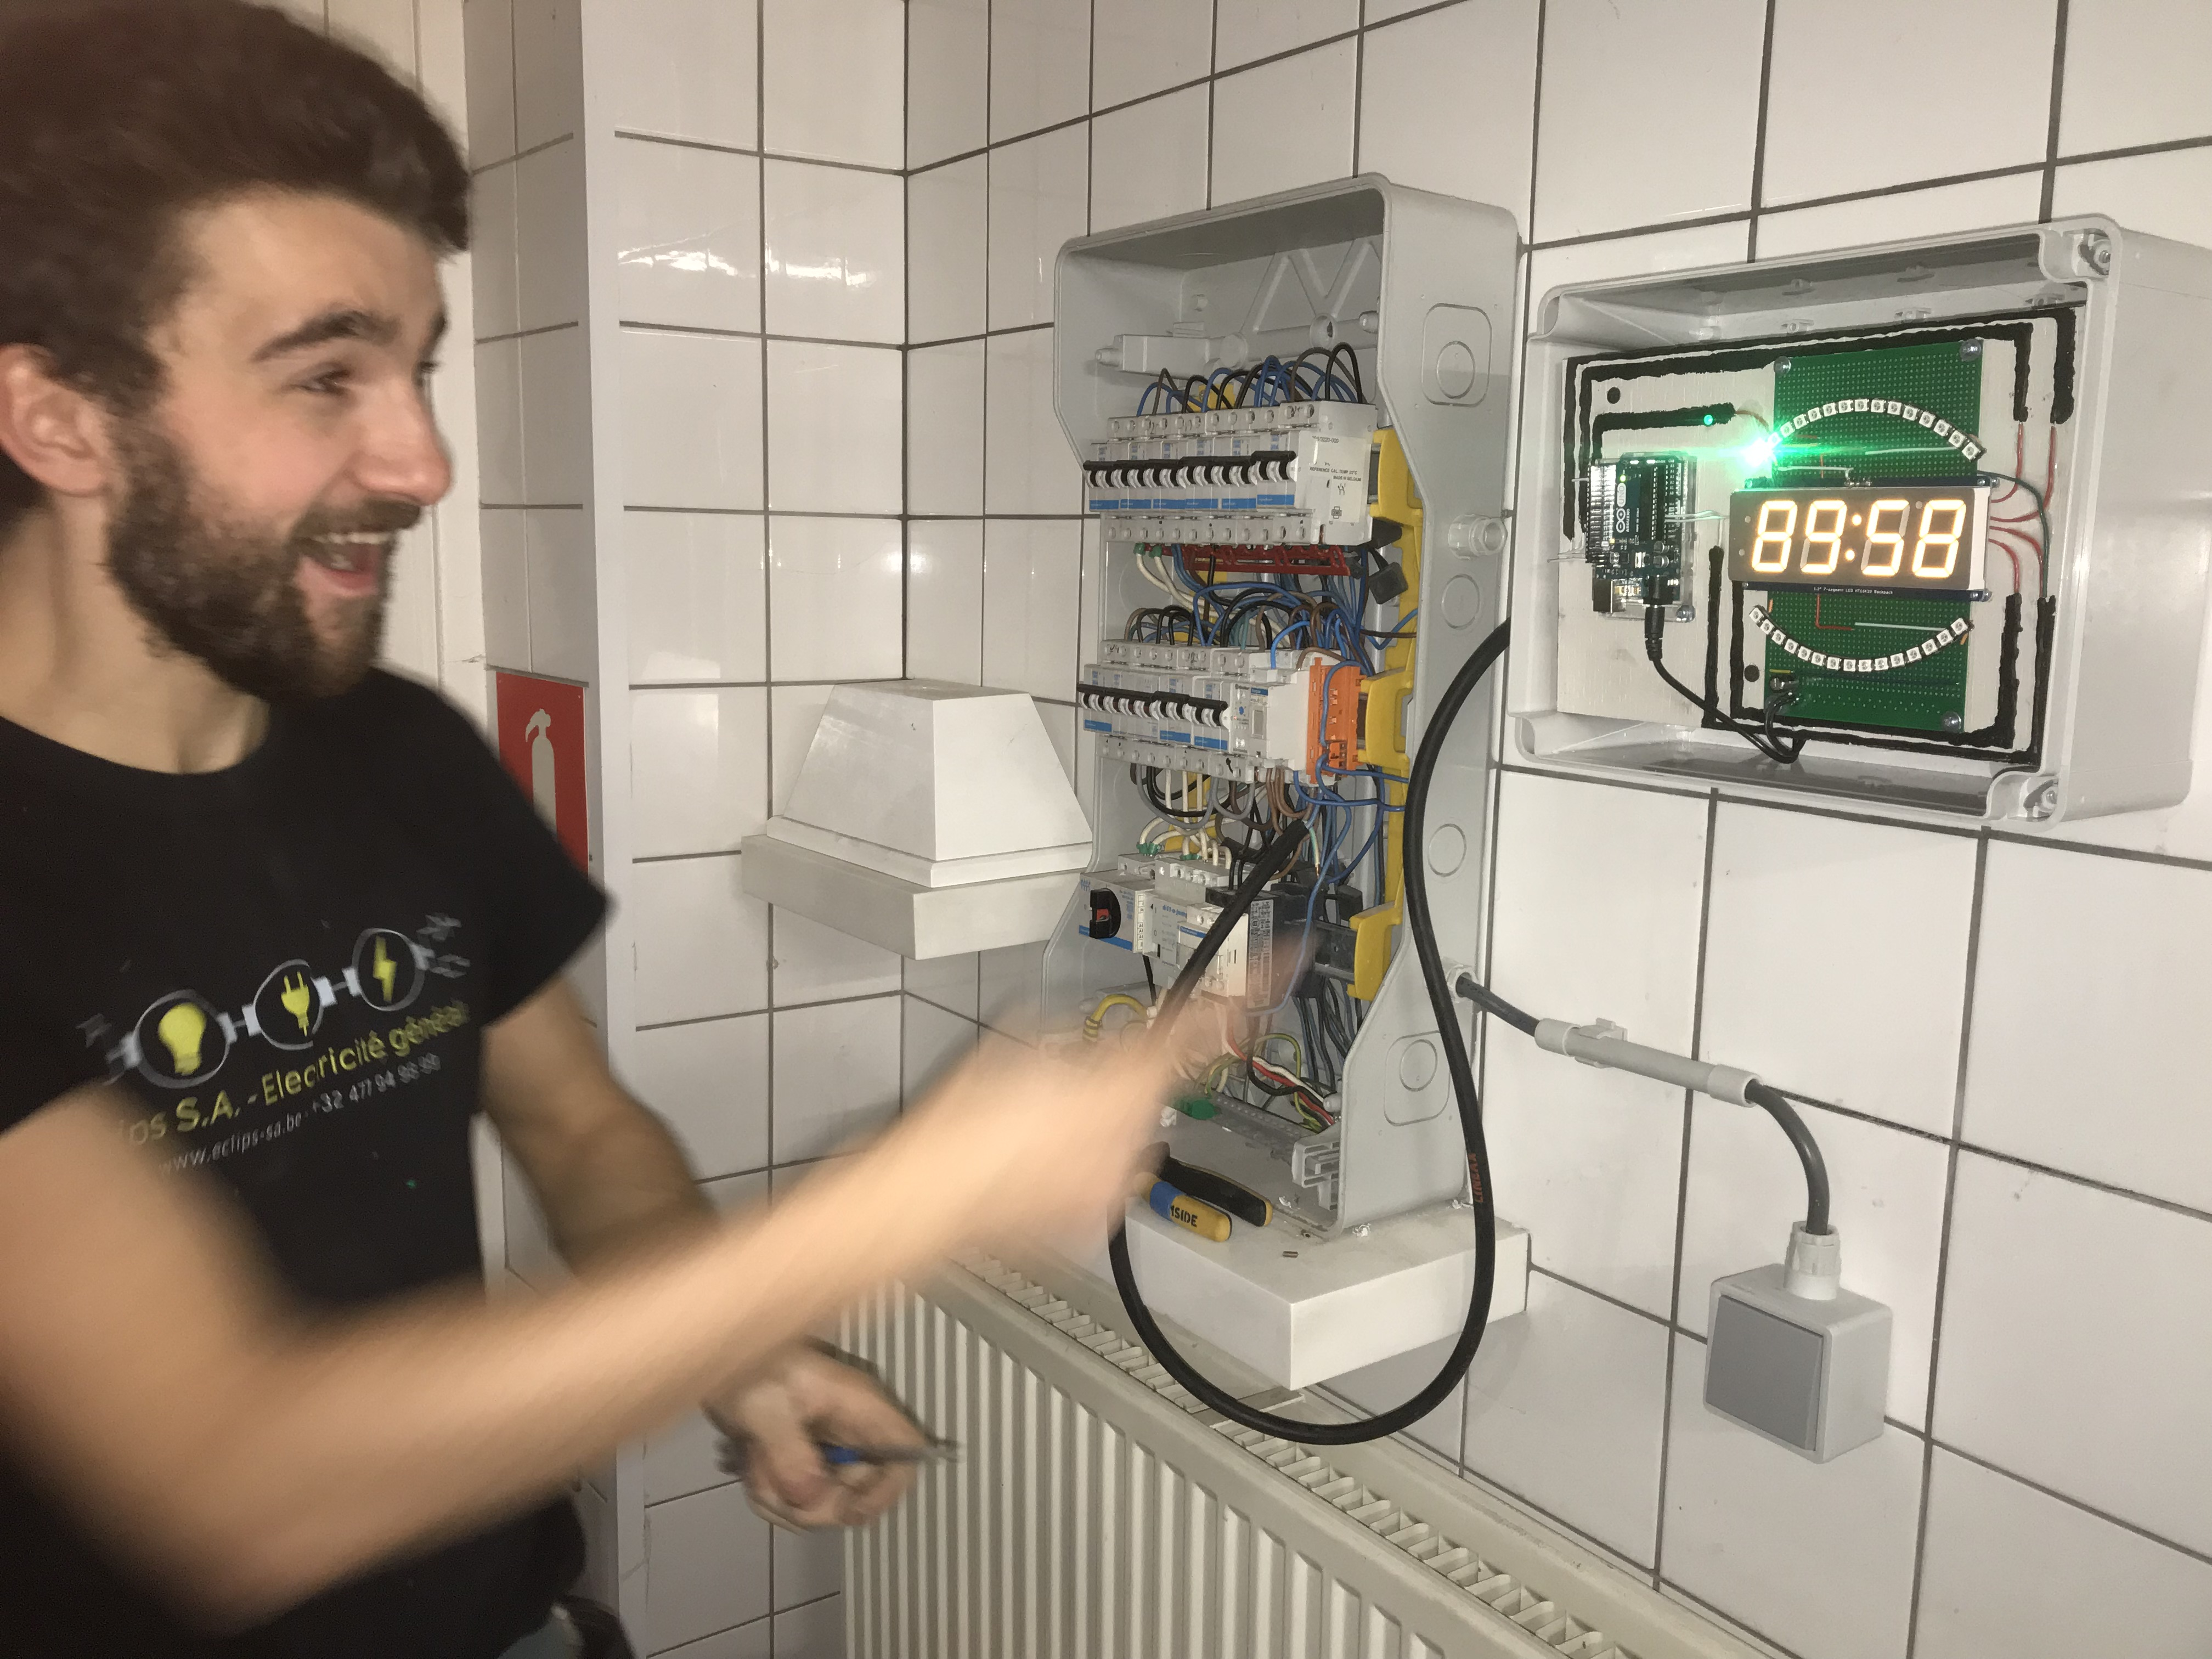
\includegraphics[height=3.6cm]{adoption.jpeg}}{Image détenue par l'auteur}} %sur la slide deux
	\hfill
	\onslide+<3->{\copyrightbox[b]{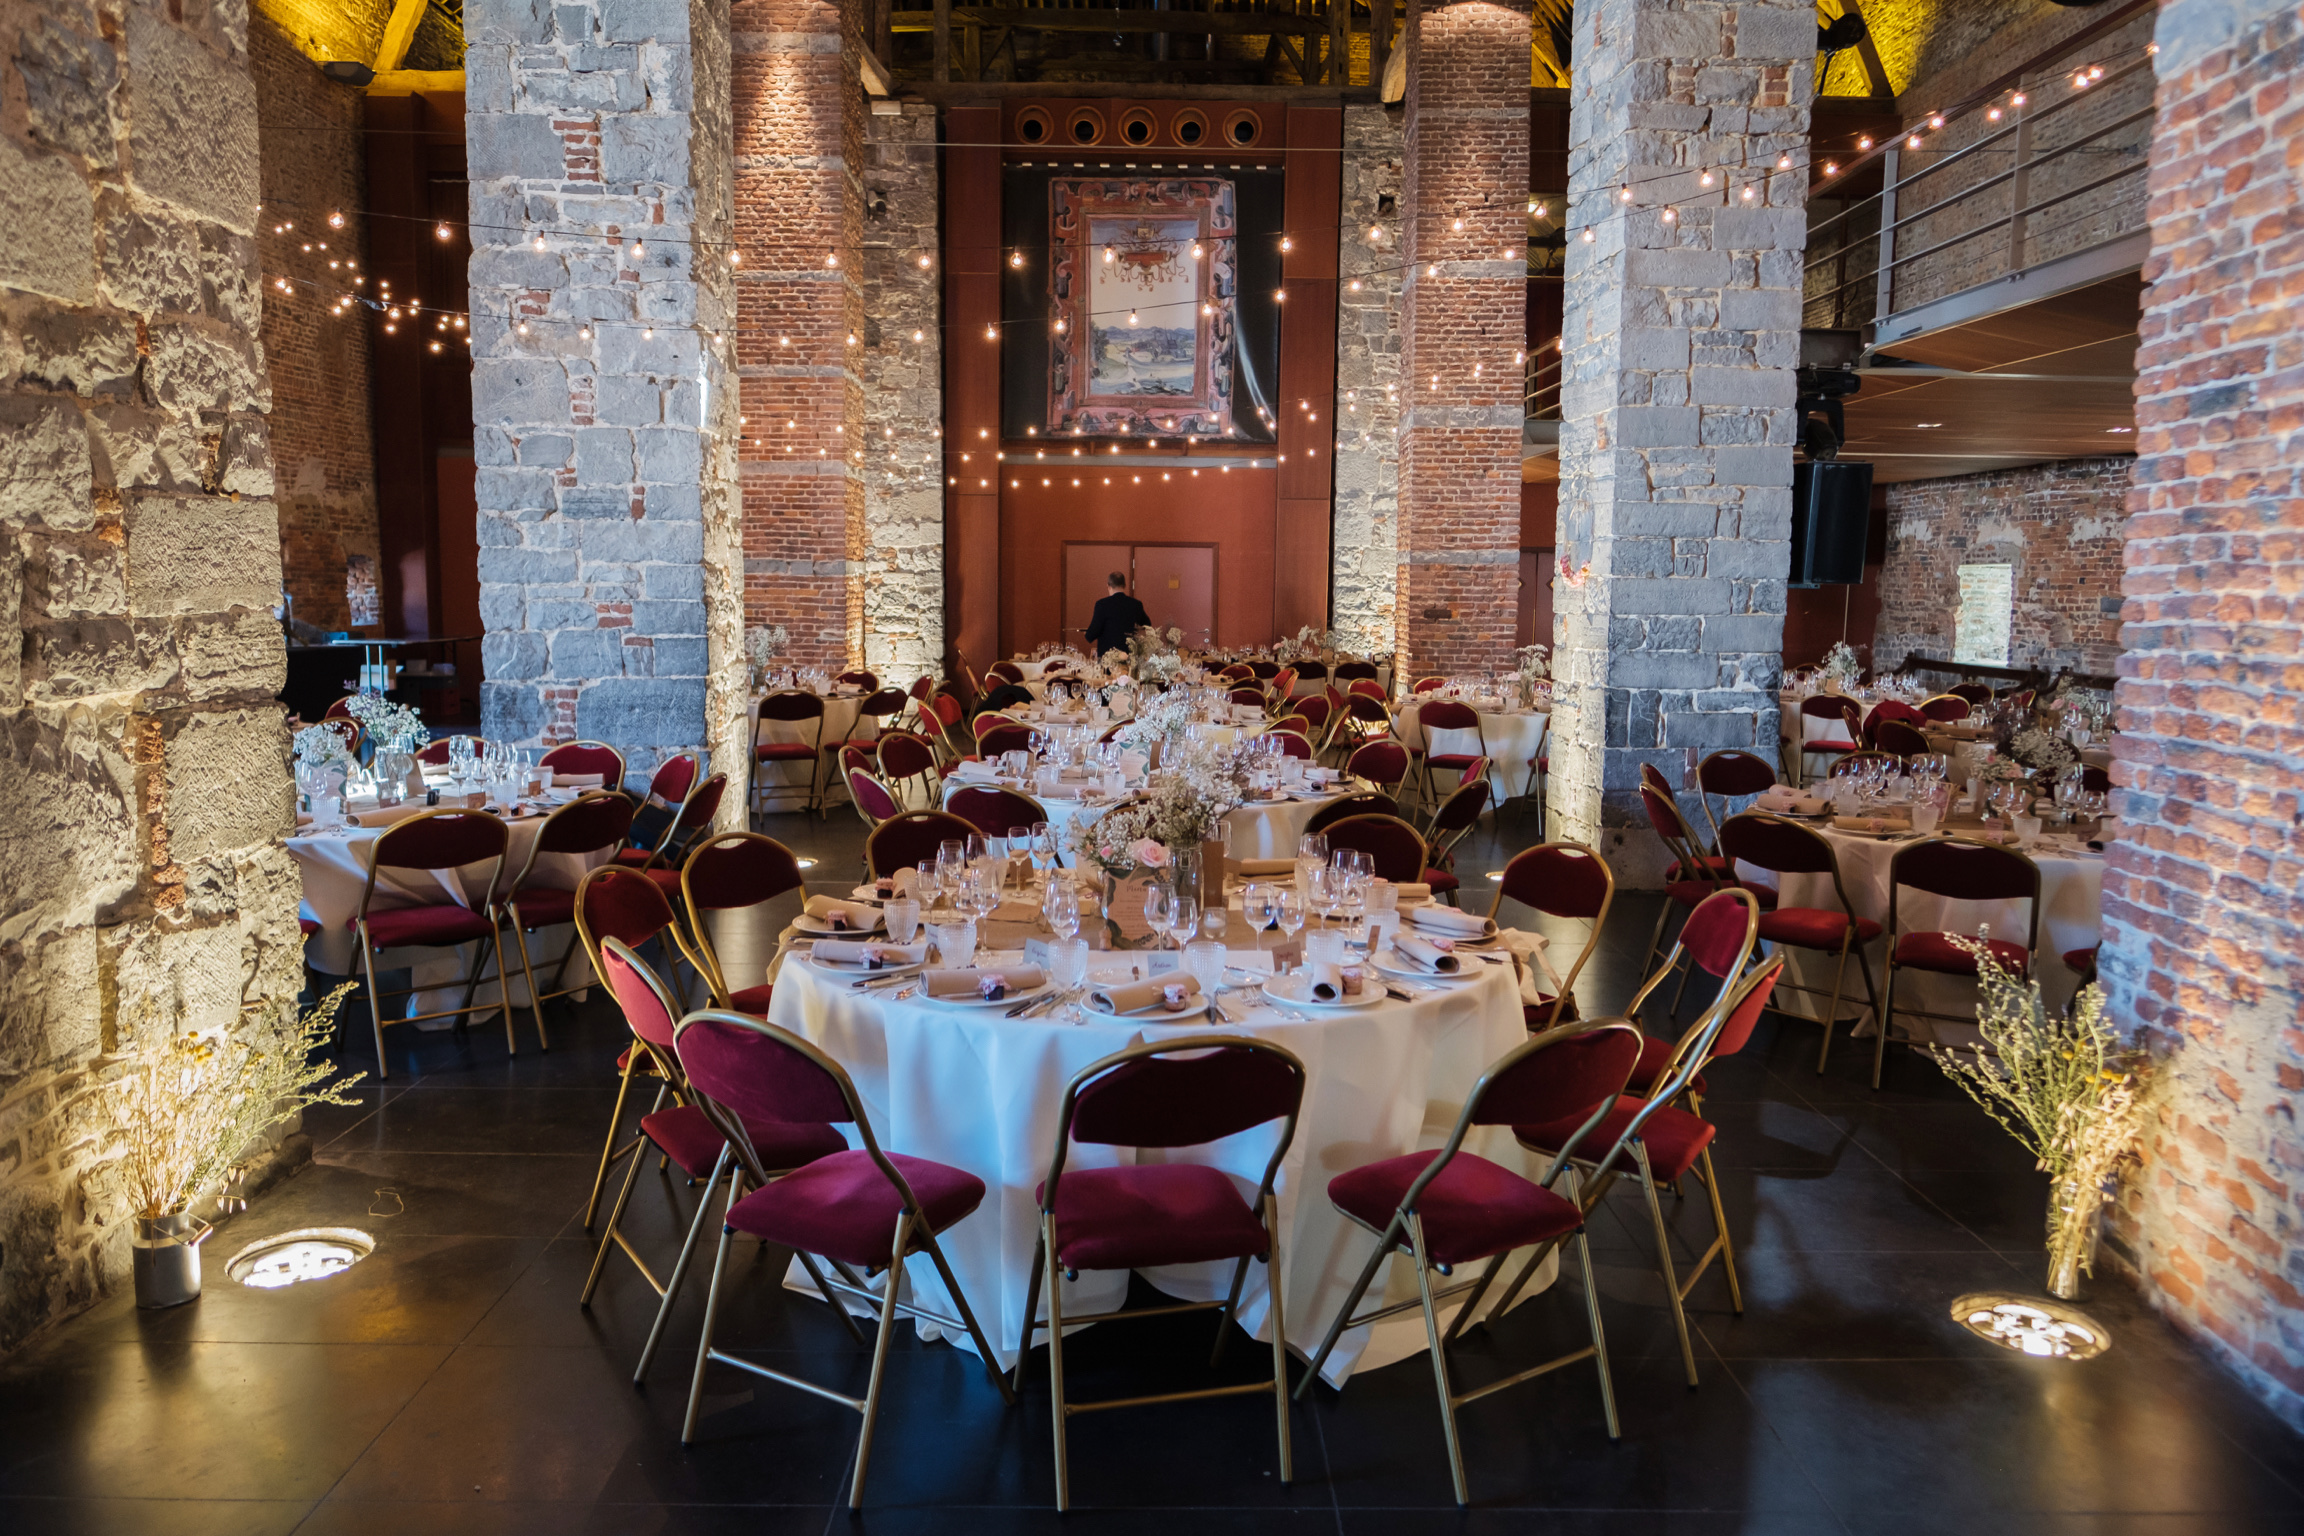
\includegraphics[height=3.6cm]{eclairage_mariage}}{Image détenue par l'auteur}} %sur la slide trois
\end{frame} 

\begin{frame}{Titre de la diapositive 14} %diapositive avec vidéo à départ automatique
\begin{center}
\movie[
	autostart,
	width=\linewidth,
	height=0.75\linewidth]
	{
\includegraphics[height=0.75\linewidth]{LED_pirate.png}}{LED_pirate.mp4}
\end{center}
\end{frame}

\section{Une conclusion}

\begin{frame}[fragile]{Titre de la diapositive 15}
      \begin{itemize}[<+- | alert@+>]
      \item Un premier truc
      \item Un deuxième truc
      \end{itemize}
\end{frame}

\section{Introduction}

\begin{frame}[fragile]{Metropolis}

  The \themename theme is a Beamer theme with minimal visual noise
  inspired by the \href{https://github.com/hsrmbeamertheme/hsrmbeamertheme}{\textsc{hsrm} Beamer
  Theme} by Benjamin Weiss.

  Enable the theme by loading

  \begin{verbatim}    \documentclass{beamer}
    \usetheme{metropolis}\end{verbatim}

  Note, that you have to have Mozilla's \emph{Fira Sans} font and XeTeX
  installed to enjoy this wonderful typography.
\end{frame}
\begin{frame}[fragile]{Sections}
  Sections group slides of the same topic

  \begin{verbatim}    \section{Elements}\end{verbatim}

  for which \themename provides a nice progress indicator \ldots
\end{frame}

\section{Title formats}

\begin{frame}{Metropolis title formats}
	\themename supports 4 different title formats:
	\begin{itemize}
		\item Regular
		\item \textsc{Small caps}
		\item \textsc{all small caps}
		\item ALL CAPS
	\end{itemize}
	They can either be set at once for every title type or individually.
\end{frame}

{
    \metroset{titleformat frame=smallcaps}
\begin{frame}{Small caps}
	This frame uses the \texttt{smallcaps} title format.

	\begin{alertblock}{Potential Problems}
		Be aware that not every font supports small caps. If for example you typeset your presentation with pdfTeX and the Computer Modern Sans Serif font, every text in small caps will be typeset with the Computer Modern Serif font instead.
	\end{alertblock}
\end{frame}
}

{
\metroset{titleformat frame=allsmallcaps}
\begin{frame}{All small caps}
	This frame uses the \texttt{allsmallcaps} title format.

	\begin{alertblock}{Potential problems}
		As this title format also uses small caps you face the same problems as with the \texttt{smallcaps} title format. Additionally this format can cause some other problems. Please refer to the documentation if you consider using it.

		As a rule of thumb: just use it for plaintext-only titles.
	\end{alertblock}
\end{frame}
}

{
\metroset{titleformat frame=allcaps}
\begin{frame}{All caps}
	This frame uses the \texttt{allcaps} title format.

	\begin{alertblock}{Potential Problems}
		This title format is not as problematic as the \texttt{allsmallcaps} format, but basically suffers from the same deficiencies. So please have a look at the documentation if you want to use it.
	\end{alertblock}
\end{frame}
}

\section{Elements}

\begin{frame}[fragile]{Typography}
      \begin{verbatim}The theme provides sensible defaults to
\emph{emphasize} text, \alert{accent} parts
or show \textbf{bold} results.\end{verbatim}

  \begin{center}becomes\end{center}

  The theme provides sensible defaults to \emph{emphasize} text,
  \alert{accent} parts or show \textbf{bold} results.
\end{frame}

\begin{frame}{Font feature test}
  \begin{itemize}
    \item Regular
    \item \textit{Italic}
    \item \textsc{Small Caps}
    \item \textbf{Bold}
    \item \textbf{\textit{Bold Italic}}
    \item \textbf{\textsc{Bold Small Caps}}
    \item \texttt{Monospace}
    \item \texttt{\textit{Monospace Italic}}
    \item \texttt{\textbf{Monospace Bold}}
    \item \texttt{\textbf{\textit{Monospace Bold Italic}}}
  \end{itemize}
\end{frame}

\begin{frame}{Lists}
  \begin{columns}[T,onlytextwidth]
    \column{0.33\textwidth}
      Items
      \begin{itemize}
        \item Milk \item Eggs \item Potatoes
      \end{itemize}

    \column{0.33\textwidth}
      Enumerations
      \begin{enumerate}
        \item First, \item Second and \item Last.
      \end{enumerate}

    \column{0.33\textwidth}
      Descriptions
      \begin{description}
        \item[PowerPoint] Meeh. \item[Beamer] Yeeeha.
      \end{description}
  \end{columns}
\end{frame}

\begin{frame}{Animation}
  \begin{itemize}[<+- | alert@+>]
    \item \alert<4>{This is\only<4>{ really} important}
    \item Now this
    \item And now this
  \end{itemize}
\end{frame}
\begin{frame}{Figures}
  \begin{figure}
    \newcounter{density}
    \setcounter{density}{20}
    \begin{tikzpicture}
      \def\couleur{alerted text.fg}
      \path[coordinate] (0,0)  coordinate(A)
                  ++( 90:5cm) coordinate(B)
                  ++(0:5cm) coordinate(C)
                  ++(-90:5cm) coordinate(D);
      \draw[fill=\couleur!\thedensity] (A) -- (B) -- (C) --(D) -- cycle;
      \foreach \x in {1,...,40}{%
          \pgfmathsetcounter{density}{\thedensity+20}
          \setcounter{density}{\thedensity}
          \path[coordinate] coordinate(X) at (A){};
          \path[coordinate] (A) -- (B) coordinate[pos=.10](A)
                              -- (C) coordinate[pos=.10](B)
                              -- (D) coordinate[pos=.10](C)
                              -- (X) coordinate[pos=.10](D);
          \draw[fill=\couleur!\thedensity] (A)--(B)--(C)-- (D) -- cycle;
      }
    \end{tikzpicture}
    \caption{Rotated square from
    \href{http://www.texample.net/tikz/examples/rotated-polygons/}{texample.net}.}
  \end{figure}
\end{frame}
\begin{frame}{Tables}
  \begin{table}
    \caption{Largest cities in the world (source: Wikipedia)}
    \begin{tabular}{@{} lr @{}}
      \toprule
      City & Population\\
      \midrule
      Mexico City & 20,116,842\\
      Shanghai & 19,210,000\\
      Peking & 15,796,450\\
      Istanbul & 14,160,467\\
      \bottomrule
    \end{tabular}
  \end{table}
\end{frame}
\begin{frame}{Blocks}
  Three different block environments are pre-defined and may be styled with an
  optional background color.

  \begin{columns}[T,onlytextwidth]
    \column{0.5\textwidth}
      \begin{block}{Default}
        Block content.
      \end{block}

      \begin{alertblock}{Alert}
        Block content.
      \end{alertblock}

      \begin{exampleblock}{Example}
        Block content.
      \end{exampleblock}

    \column{0.5\textwidth}

      \metroset{block=fill}

      \begin{block}{Default}
        Block content.
      \end{block}

      \begin{alertblock}{Alert}
        Block content.
      \end{alertblock}

      \begin{exampleblock}{Example}
        Block content.
      \end{exampleblock}

  \end{columns}
\end{frame}
\begin{frame}{Math}
  \begin{equation*}
    e = \lim_{n\to \infty} \left(1 + \frac{1}{n}\right)^n
  \end{equation*}
\end{frame}
\begin{frame}{Line plots}
  \begin{figure}
    \begin{tikzpicture}
      \begin{axis}[
        mlineplot,
        width=0.9\textwidth,
        height=6cm,
      ]

        \addplot {sin(deg(x))};
        \addplot+[samples=100] {sin(deg(2*x))};

      \end{axis}
    \end{tikzpicture}
  \end{figure}
\end{frame}
\begin{frame}{Bar charts}
  \begin{figure}
    \begin{tikzpicture}
      \begin{axis}[
        mbarplot,
        xlabel={Foo},
        ylabel={Bar},
        width=0.9\textwidth,
        height=6cm,
      ]

      \addplot plot coordinates {(1, 20) (2, 25) (3, 22.4) (4, 12.4)};
      \addplot plot coordinates {(1, 18) (2, 24) (3, 23.5) (4, 13.2)};
      \addplot plot coordinates {(1, 10) (2, 19) (3, 25) (4, 15.2)};

      \legend{lorem, ipsum, dolor}

      \end{axis}
    \end{tikzpicture}
  \end{figure}
\end{frame}
\begin{frame}{Quotes}
  \begin{quote}
    Veni, Vidi, Vici
  \end{quote}
\end{frame}

{%
\setbeamertemplate{frame footer}{My custom footer}
\begin{frame}[fragile]{Frame footer}
    \themename defines a custom beamer template to add a text to the footer. It can be set via
    \begin{verbatim}\setbeamertemplate{frame footer}{My custom footer}\end{verbatim}
\end{frame}
}

\begin{frame}{References}
  Some references to showcase [allowframebreaks] \cite{knuth92,ConcreteMath,Simpson,Er01,greenwade93}
\end{frame}

\section{Conclusion}

\begin{frame}{Summary}

  Get the source of this theme and the demo presentation from

  \begin{center}\url{github.com/matze/mtheme}\end{center}

  The theme \emph{itself} is licensed under a
  \href{http://creativecommons.org/licenses/by-sa/4.0/}{Creative Commons
  Attribution-ShareAlike 4.0 International License}.

  \begin{center}\ccbysa\end{center}

\end{frame}

\begin{frame}[standout]
  Questions?
\end{frame}

\appendix

\begin{frame}[fragile]{Backup slides}
  Sometimes, it is useful to add slides at the end of your presentation to
  refer to during audience questions.

  The best way to do this is to include the \verb|appendixnumberbeamer|
  package in your preamble and call \verb|\appendix| before your backup slides.

  \themename will automatically turn off slide numbering and progress bars for
  slides in the appendix.
\end{frame}

\begin{frame}[allowframebreaks]{References}

  \bibliography{demo}
  \bibliographystyle{abbrv}

\end{frame}

\end{document}
